% =============================================================================
%  VI. RESULTS — COHORT AND LABEL VARIANCE
% =============================================================================
\begin{frame}{VI. Results --- Cohort and Label Variance}
\begin{center}\tablestyle
\begin{tabular}{clccc}
\toprule
\textbf{Variant} & \textbf{Name} & \textbf{ICU Stays}
  & \textbf{Sepsis Cases} & \textbf{\%} \\
\midrule
A & Narrow           & 65,078 & 6,252              & 9.6\% \\
B & Seymour-Standard & 65,078 & 6,447              & 9.9\% \\
C & Liberal          & 65,078 & \textbf{12,581}     & \textbf{19.3\%} \\
\bottomrule
\end{tabular}
\end{center}

\vspace{8pt}
The Liberal definition found almost \textbf{2$\times$ more sepsis cases}
than the other two definitions.

\vspace{4pt}
The patient data and database were the same. Only the way sepsis was defined
was different.
\end{frame}


% =============================================================================
%  VI. RESULTS — H1: LABEL vs MODEL
% =============================================================================
\begin{frame}{VI. Results --- H1: Label Has More Impact Than Model \confirmed}
\begin{atucols}[c]

\begin{column}{0.46\textwidth}
  \centering
  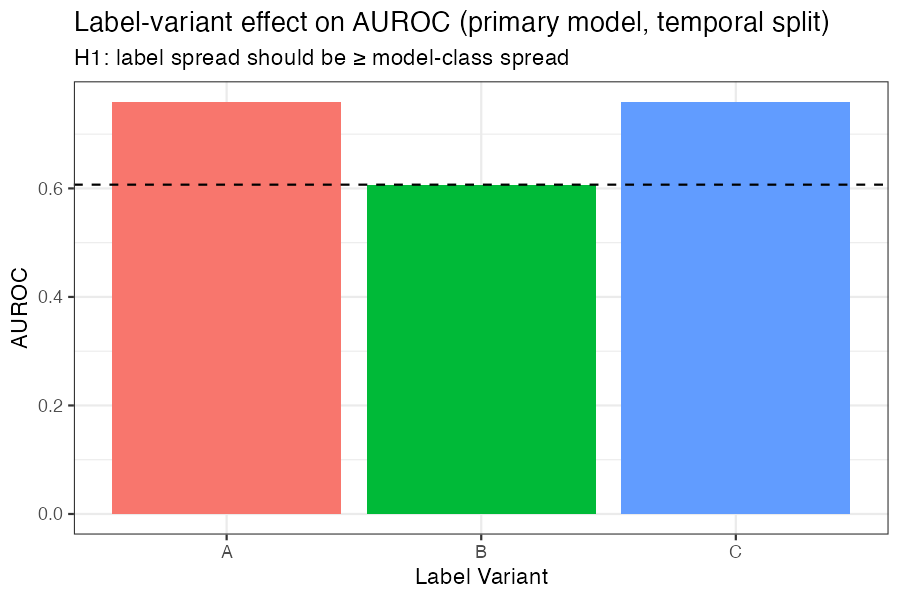
\includegraphics[width=\columnwidth]{images/09_label_variance_auroc.png}
\end{column}

\begin{column}{0.52\textwidth}
  \begin{itemize}
    \item \textbf{Label variation:} AUROC changed by \textbf{0.153} when the
          sepsis definition changed while using the same model.
    \item \textbf{Model variation:} AUROC changed by \textbf{0.145} when the
          model changed while using the same label.
    \item This confirms Cohen et al.'s~\cite{cohen2024subtle} finding that
          sepsis label definition can strongly influence model performance.
  \end{itemize}
  \vspace{4pt}
  \begin{alertblock}{}
    The way sepsis is defined can affect performance as much as, or more
    than, the AI model itself.
  \end{alertblock}
\end{column}

\end{atucols}
\end{frame}


% =============================================================================
%  VI. RESULTS — H2: COEFFICIENT INSTABILITY
% =============================================================================
\begin{frame}{VI. Results --- H2: Coefficient Instability \confirmed}
\begin{itemize}
  \item \textbf{10 out of 25 features} changed their effect or strength
        significantly across different sepsis label definitions.
  \item Affected features include: MAP, temperature, bilirubin, platelets,
        vasopressors, norepinephrine/epinephrine, respiratory rate change,
        platelet measurement, WBC measurement, and P/F ratio.
\end{itemize}

\vspace{6pt}
\begin{block}{Implication}
  A published hazard ratio for MAP could show a positive, negative, or
  almost no association with sepsis risk depending only on how the
  antibiotic-culture time window is defined~\cite{lauritsen2021framing}.
\end{block}

\vspace{6pt}
\textbf{Feature effects cannot be reliably interpreted without knowing which
sepsis label definition was used.}
\end{frame}


% =============================================================================
%  VI. RESULTS — H3: TREATMENT LEAKAGE
% =============================================================================
\begin{frame}{VI. Results --- H3: Treatment Leakage \confirmed}
The treatment-anchored window~\cite{kamran2024evaluation} uses only
information available \textbf{before the first antibiotic or blood culture}.

\vspace{6pt}
\begin{atucols}[c]

\begin{column}{0.40\textwidth}
\begin{center}\tablestyle
\begin{tabular}{lc}
\toprule
\textbf{Metric} & \textbf{Value} \\
\midrule
Patient-hours analysed & 179,003 \\
Sepsis onset events    & \textbf{0} \\
\bottomrule
\end{tabular}
\end{center}
\end{column}

\begin{column}{0.58\textwidth}
\begin{alertblock}{Critical Finding}
  No sepsis onset event is found before the clinical actions used to define
  the Sepsis-3 label.
\end{alertblock}
\end{column}

\end{atucols}

\vspace{6pt}
This is not just a small drop in model performance (0.03 AUROC). The
prediction target is \textbf{completely missing} in the clinically realistic
time window.

\vspace{4pt}
\textbf{Most MIMIC-IV sepsis prediction models are learning when doctors
suspect sepsis and start treatment, rather than detecting when a patient's
health is starting to get worse.}
\end{frame}


% =============================================================================
%  VI. RESULTS — H4: SPLIT OPTIMISM
% =============================================================================
\begin{frame}{VI. Results --- H4: Split Optimism \confirmed}
\begin{center}\tablestyle
\begin{tabular}{llcc}
\toprule
\textbf{Split} & \textbf{Model} & \textbf{AUROC} & \textbf{Utility Score} \\
\midrule
Temporal & Primary & 0.607 & --1.004 \\
Random   & Primary & 0.730 & --1.000 \\
Temporal & GBT     & 0.746 & --4.849 \\
Random   & GBT     & 0.720 & --5.167 \\
\bottomrule
\end{tabular}
\end{center}

\vspace{6pt}
\begin{itemize}
  \item \textbf{Primary model:} Random-split AUROC was \textbf{0.123 higher}
        than temporal-split AUROC (threshold: $\geq$ 0.02).
  \item The random split lets future patient patterns leak into training,
        inflating reported performance.
  \item This confirms Guo et al.'s~\cite{guo2022temporal} finding:
        \textbf{studies using random splits may overestimate real-world
        performance.}
\end{itemize}
\end{frame}


% =============================================================================
%  VI. RESULTS — H5: EXTERNAL VALIDATION
% =============================================================================
\begin{frame}{VI. Results --- H5: External Validation on
              eICU-CRD~\cite{pollard2018eicu}}
\begin{center}\tablestyle
\begin{tabular}{llccc}
\toprule
\textbf{Variant} & \textbf{Model}
  & \textbf{AUROC (eICU)} & \textbf{AUROC (MIMIC)} & \textbf{Drop} \\
\midrule
A   & Primary & 0.736          & 0.760 & 0.024 \\
B   & Primary & \textbf{0.437} & 0.607 & \textbf{0.170} \\
C   & Primary & 0.725          & 0.759 & 0.034 \\
--- & NEWS2   & 0.605          & 0.63  & 0.025 \\
\bottomrule
\end{tabular}
\end{center}

\vspace{6pt}
\begin{itemize}
  \item Variants A and C showed similar performance on both datasets, with
        only small drops.
  \item \textbf{Variant B (Seymour-Standard) showed a large performance drop
        of 0.170 AUROC} when tested on eICU-CRD.
  \item The most commonly used sepsis label definition did not transfer well
        to a different hospital dataset.
\end{itemize}
\end{frame}


% =============================================================================
%  VI. RESULTS — H6: MODEL-CLASS DIFFERENCE
% =============================================================================
\begin{frame}{VI. Results --- H6: Model-Class Difference \rejected}
\begin{atucols}[c]

\begin{column}{0.46\textwidth}
  \centering
  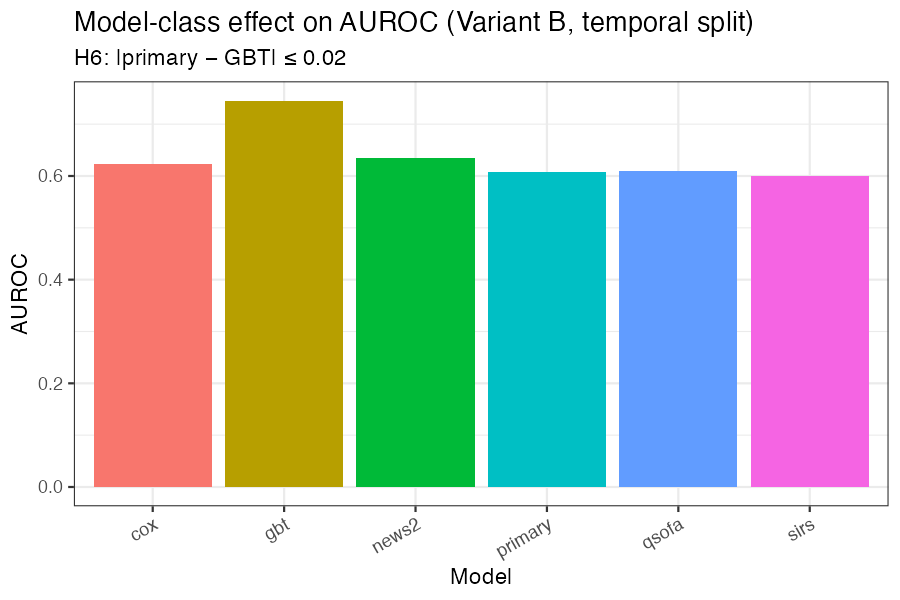
\includegraphics[width=\columnwidth]{images/09_model_class_auroc.png}
\end{column}

\begin{column}{0.52\textwidth}
  \begin{itemize}
    \item \textbf{GBT AUROC:} 0.746
    \item \textbf{Primary Model AUROC:} 0.607
    \item Difference: \textbf{0.139}
  \end{itemize}
  \vspace{4pt}
  \begin{itemize}
    \item \textbf{GBT Utility Score:} --4.849
    \item \textbf{Primary Utility Score:} --1.004
  \end{itemize}
  \vspace{6pt}
  \begin{alertblock}{}
    The model ranking changes depending on the evaluation metric. A model
    that looks better by AUROC may perform worse in real clinical use.
  \end{alertblock}
\end{column}

\end{atucols}
\end{frame}


% =============================================================================
%  VI. RESULTS — INTERNAL PERFORMANCE
% =============================================================================
\begin{frame}{VI. Results --- Internal Performance (Temporal Test)}
\begin{center}\tablestyle\footnotesize
\begin{tabular}{llccc}
\toprule
\textbf{Variant} & \textbf{Model} & \textbf{AUROC}
  & \textbf{Utility Score} & \textbf{Alert Burden} \\
\midrule
A   & Primary & 0.760 & \textbf{--1.000}  & $\infty$ \\
A   & GBT     & 0.742 & --4.667           & 203 \\
B   & Primary & 0.607 & --1.004           & $\infty$ \\
B   & \textbf{GBT} & \textbf{0.746} & --4.849 & 194 \\
C   & Primary & 0.759 & --1.000           & $\infty$ \\
C   & GBT     & 0.752 & --2.475           & 93 \\
--- & NEWS2   & 0.63--0.64 & --1.1 to --1.6 & 97--223 \\
\bottomrule
\end{tabular}
\end{center}

\vspace{4pt}
\textbf{All models had a negative Utility Score}, meaning they did not
provide clinical benefit and performed worse than giving no alerts.

\vspace{2pt}
\textbf{Alert burden:} For every real sepsis alert, the system generated
\textbf{93--359 false alerts} (benchmark: 1.4~\cite{moor2023review}).
\end{frame}


% =============================================================================
%  VI. RESULTS — EQUITY ANALYSIS
% =============================================================================
\begin{frame}{VI. Results --- Equity Analysis \novelfinding}
\begin{atucols}[c]

\begin{column}{0.44\textwidth}
  \centering
  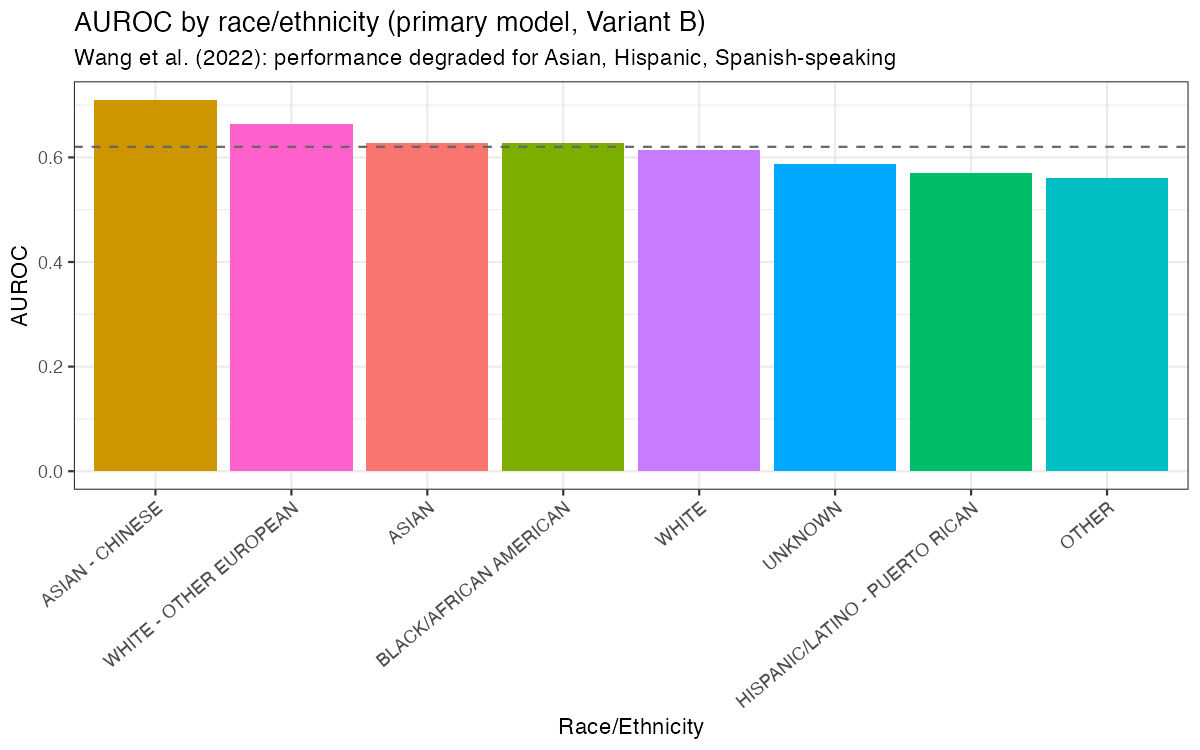
\includegraphics[width=\columnwidth]{images/10_auroc_by_race.png}
\end{column}

\begin{column}{0.54\textwidth}
  \begin{itemize}
    \item AUROC varied by up to \textbf{0.15} across racial subgroups
          (primary model, Variant~B), from 0.56 (Other) to 0.71
          (Asian-Chinese).
    \item The percentage of patients labelled as septic changed by
          \textbf{7.4--14.2 percentage points} across different label
          definitions within demographic subgroups.
    \item The \textbf{Unknown/Unable-to-obtain} race groups showed the
          largest changes (12.3--12.8\,pp).
    \item This is the first study to examine both model performance
          disparities and label sensitivity across
          subgroups~\cite{wang2022equity}.
  \end{itemize}
\end{column}

\end{atucols}
\end{frame}


% =============================================================================
%  VI. RESULTS — VARIANCE DECOMPOSITION SUMMARY
% =============================================================================
\begin{frame}{VI. Results --- Variance Decomposition Summary}
\begin{center}\tablestyle
\begin{tabular}{lccc}
\toprule
\textbf{Factor} & \textbf{AUROC Change}
  & \textbf{Related Hypothesis} & \textbf{Status} \\
\midrule
Sepsis label definition
  & 0.153 & H1 & \textcolor{BabyMint!60!green}{\textbf{CONFIRMED}} \\
Model choice
  & 0.145 & H6 & \textcolor{BabyPink!70!red}{\textbf{REJECTED}} \\
Split method (temporal vs random)
  & 0.123 & H4 & \textcolor{BabyMint!60!green}{\textbf{CONFIRMED}} \\
Evaluation metric (AUROC vs Utility Score)
  & 0.170 & H5 & --- \\
\bottomrule
\end{tabular}
\end{center}

\vspace{8pt}
\textbf{All four analyst decisions create AUROC changes of 0.12--0.17.}

\vspace{4pt}
Most studies fix one sepsis label and compare models. This measures only one
source of variation while ignoring three other sources of similar importance.
\end{frame}
